%%%%%%%%%%%%%%%%%%%%%%%%%%%%%%%%%%%%%%%%%%%%%%%%%%%%%%%%%%%%%%%%%%
%%This presentation was fullly copied from the WSC presentation (dec. 2015)
%% and addapted for the CAA2k16
\documentclass[12pt, handout=show,notes=show]{beamer}
\usetheme[width=0cm]{Goettingen}
\usecolortheme{rose}
\useoutertheme{default}
\setbeamerfont{caption}{size=\scriptsize}

\addtobeamertemplate{navigation symbols}{}{%
	\usebeamerfont{footline}%
	\usebeamercolor[fg]{footline}%
	\hspace{1em}%
	$\dfrac{\insertframenumber}{\inserttotalframenumber}$
}

\usepackage{hyperref}
\usepackage{fontspec} 
\setsansfont{Futura LT}
%\setmonofont[Scale=0.8]{Monaco} 


\usepackage{arydshln}

\usepackage{amsmath}

\usepackage{mathptmx}
\usepackage{latexsym}
\usepackage{mathtools}
\usepackage{multirow}
\usepackage{caption}


\DeclarePairedDelimiter\abs{\lvert}{\rvert}%
\DeclarePairedDelimiter\norm{\lVert}{\rVert}%


\makeatletter
\let\oldabs\abs
\def\abs{\@ifstar{\oldabs}{\oldabs*}}
\let\oldnorm\norm
\def\norm{\@ifstar{\oldnorm}{\oldnorm*}}
\makeatother

\title{
	CAA2016\\
	Co-evolution of trade and culture\\
	Impact of cultural network topology on economic dynamics.
}

\institute{31 March 2016}

\author{Simon Carrignon, Jean-Marc Montanier, Jérôme Michaud \& Xavier Rubio-Campillo}

\date{
	\scriptsize
	\begin{columns}
		\begin{column}{.3\textwidth}
			\begin{center}
				Barcelona Supercomputing Center	\\
				
\includegraphics[height=1cm]{images/bscLogo.jpg} \hspace{2cm}
			\end{center}
		\end{column}
		\begin{column}{.3\textwidth}
			\begin{center}
				Univ. Pompeu Fabra Complex System Lab.\\
				\includegraphics[height=1cm]{images/upfLogo.jpeg} %declare logo image with an alias here 
			\end{center}
		\end{column}
	\end{columns}

}
\begin{document}
\begin{frame}
	\maketitle

\end{frame}

\begin{frame}{Plan of the presentation}
	\begin{enumerate}
		\item Introduction
			\vfill
		\item Model Description
			\vfill
		\item Experimental Setup \& Results
			\vfill
		\item Case Study: Rome
			\vfill
	\end{enumerate}
	
\end{frame}

\section{Introduction}
\begin{frame}{Cultural Evolution}
	\begin{center}
		\includegraphics[width=.4\textwidth]{images/beardevo.jpg} 
	\end{center}
	How Cultural Traits Evolve?
\end{frame}

\begin{frame}{Cultural Evolution}
	\begin{center}
		\includegraphics[width=4cm]{images/dalmatian.jpg} \hspace{2cm}
		\includegraphics[width=2cm]{images/pottery.jpg}\\
		\vspace{1cm}
		\includegraphics[width=4cm]{images/name.jpg}
	\end{center}
	Similar variants distributions
	\begin{figure}
		\begin{columns}
			\begin{column}{.8\textwidth}
				\centering
				\includegraphics[width=.6\textwidth]{images/powerlawrepartition.jpg}
			\end{column}
			\begin{column}{.3\textwidth}
				\tiny
				Square: male names\\
				Circle: female names\\
			From Bentley et al,~2004.
			\end{column}
		\end{columns}
	\end{figure}
\end{frame}

\begin{frame}{What Generate Those Cultural changes?}
	Simple mechanisms (Bentley et al, 2004):
	\begin{itemize}
		\item Random Copy 
		\item Frequency biased (conformist/anti-conformist\dots)
		\item \dots	
	\end{itemize}
	\begin{figure}
		\begin{columns}
			\begin{column}{.8\textwidth}
				\centering
				\includegraphics[width=.6\textwidth]{images/powerlawrepartition.jpg}
			\end{column}
			\begin{column}{.3\textwidth}
				\tiny
				Square: male names\\
				Circle: female names\\
				Dotted and plain lines: model result with different copy probabilities.\\
			From Bentley et al,~2004.
			\end{column}
		\end{columns}
	\end{figure}
\end{frame}

\section{Context}



\begin{frame}{Trade and Cultural Network}
    Traded Cultural Artificat : 
    \begin{columns}
	\begin{column}{.5\textwidth}
	    \includegraphics[width=\textwidth]{images/obsidianFlint.jpg}	
	\end{column}
	\begin{column}{.4\textwidth}
	    \small
	    Non-neutral value (utility): 
	    \begin{itemize}
		\item ``Usefulness''
		\item popularity
		\item availability
		\item \dots
	    \end{itemize}
	\end{column}
    \end{columns}
\end{frame}

\begin{frame}
	\begin{center}
		What happen when such mechanisms act on traits impacting economy?
	\end{center}
	\begin{columns}
		\begin{column}{.3\textwidth}
			\includegraphics[width=\textwidth]{images/bordeaux.jpg}	
		\end{column}
		\begin{column}{.2\textwidth}
		\end{column}
		\begin{column}{.3\textwidth}
			\includegraphics[width=3cm]{images/napa}	
		\end{column}
	\end{columns}
\end{frame}

\begin{frame}{Co-evolution of Economy and Culture}

	%How Simple Cultural Dynamics influence Economy That in turn will influence cultural dynamics.

	\begin{alertblock}{Interaction between Culture and Economy}
	    \begin{center}
		Cultural mechanisms transform Economy \\
		\begin{center}
		    $  \scalebox{3}{\circlearrowright}$
		\end{center}
		Economy influences Culture
	    \end{center}
	\end{alertblock}


\end{frame}

\section{ABM Framework}

\begin{frame}{A General Agent Based Framework }
	\begin{center}
	    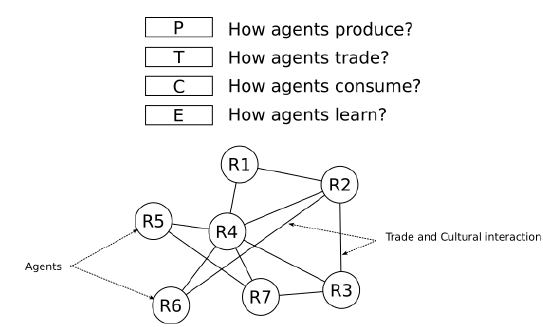
\includegraphics[width=.6\textwidth]{images/schema_model.png}
	\end{center}
\end{frame}



\begin{frame}{A General Agent Based Framework }

     Two main components:
     \vfill
    \begin{enumerate}
	\item Economic side: Bartering Economy (Gintis 2009),
		\vspace{1cm}
	\item Cultural side: ``copy the most successful'' (Bentley 2006).
    \end{enumerate}
\end{frame}
	
\begin{frame}{The Model}
	\begin{block}{1. The Economy \& the Barter Mechanism}
	    \begin{itemize}
		    \item $N$ goods
		\item $M$ Agent 
		    $\left\{
			\begin{tabular}{@{}l@{}}
			    a quantity of each Goods \\
			    $N$ values attributed to each goods\\
			\end{tabular}
			\right.$
		    \item Agents \emph{produce} one good and \emph{exchange} it to obtain the other goods.
		    \item After the exchange, the agents \emph{consume} all goods 
		\end{itemize}

	\end{block}
\end{frame}

\begin{frame}{The Model}
	\begin{block}{2. Cultural Mechanisms}
	    Every step:
	    \begin{itemize}
		    \item Economic activity (cf. previous slide).
		    \item A \emph{score} is given following $f(q_n)$  a shared \& fixed ``utility function''.
	    \end{itemize}
		After 10 steps:
		\begin{itemize}
		    \item Less successful agents \emph{copy} the most successful (Biased-Copy).
		    \item Given a probability $\mu$ the value attributed to some goods is modified (Innovation/Mutation)
		\end{itemize}
	\end{block}
\end{frame}

\begin{frame}{The Model }
	\begin{figure}
	    \caption{Example for 3 goods and 500 agents}
	    \begin{columns}
		\column{.5\textwidth}
		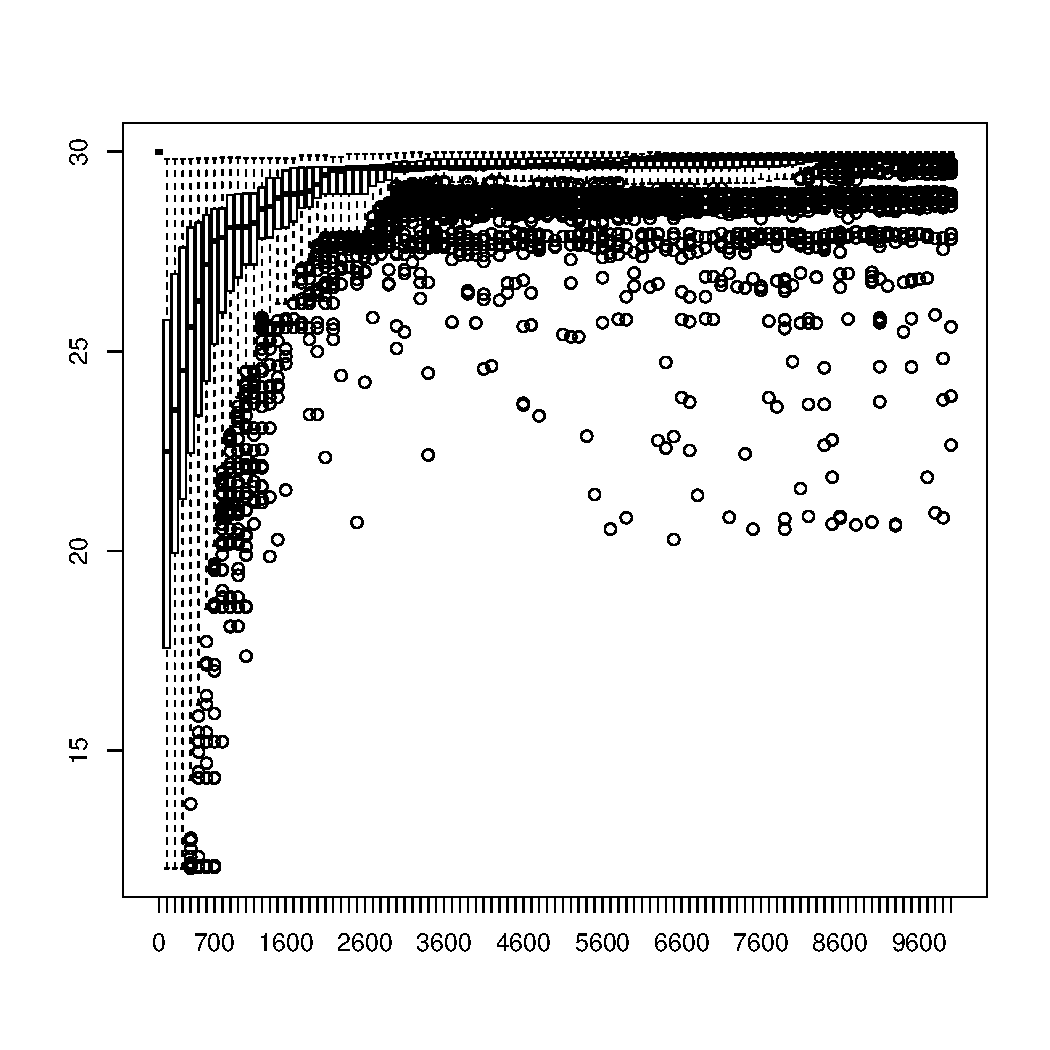
\includegraphics[height=\textwidth]{images/ScoreEvolutionForD-G3N500.pdf}\\
	    \end{columns}
		@~Equilibrium: mean of score  $\rightarrow$ score max.
	\end{figure}
	
\end{frame}

\section{Experimental Setup \& Results}
\begin{frame}{Experiments}
	\textbf{Impact of the topologie of the cultural network }
	$\rightarrow$ Average Length Path vs Density:\\
	\begin{center}
	    ``What properties of the cultural network influe on the economic dynamics? '' 
	\end{center}




\end{frame}

\begin{frame}{Experimental Setup}
	Set of networks with combinaison of properties:
	\begin{itemize}
	    \item Density of the network (D)
	    \item Average Length Path (A)
	\end{itemize}

    \begin{table}

	\centering
	\begin{tabular}{l|ccc}
	    	 	& $D_1$	 	& \dots & $D_n$		\\\hline
	    $A_1$	& $Net_{11}$	& 	& $Net_{1n}$	\\	
	    \dots	&		&\dots	&		\\
	    $A_m$	& $Net_{m1}$	& 	& $Net_{mn}$	\\	
	\end{tabular}
	\label{tab:net}
    \end{table}
\end{frame}
%	\\Trade Mechanism + Success Biased Copy\\
%	\vfill
%	vs\\
%	\vfill
%	\textbf{Neutral Model}\\ Trade Mechanism + Random Copy\\
	 
\begin{frame}{Experimental Setup}
    \begin{table}
	\centering
	\begin{tabular}{lccc}
	    	&$D=0.02$ & $D=0.04$\\
		$A\approx17$&
		\includegraphics[width=2.5cm]{images//g02.pdf}&
		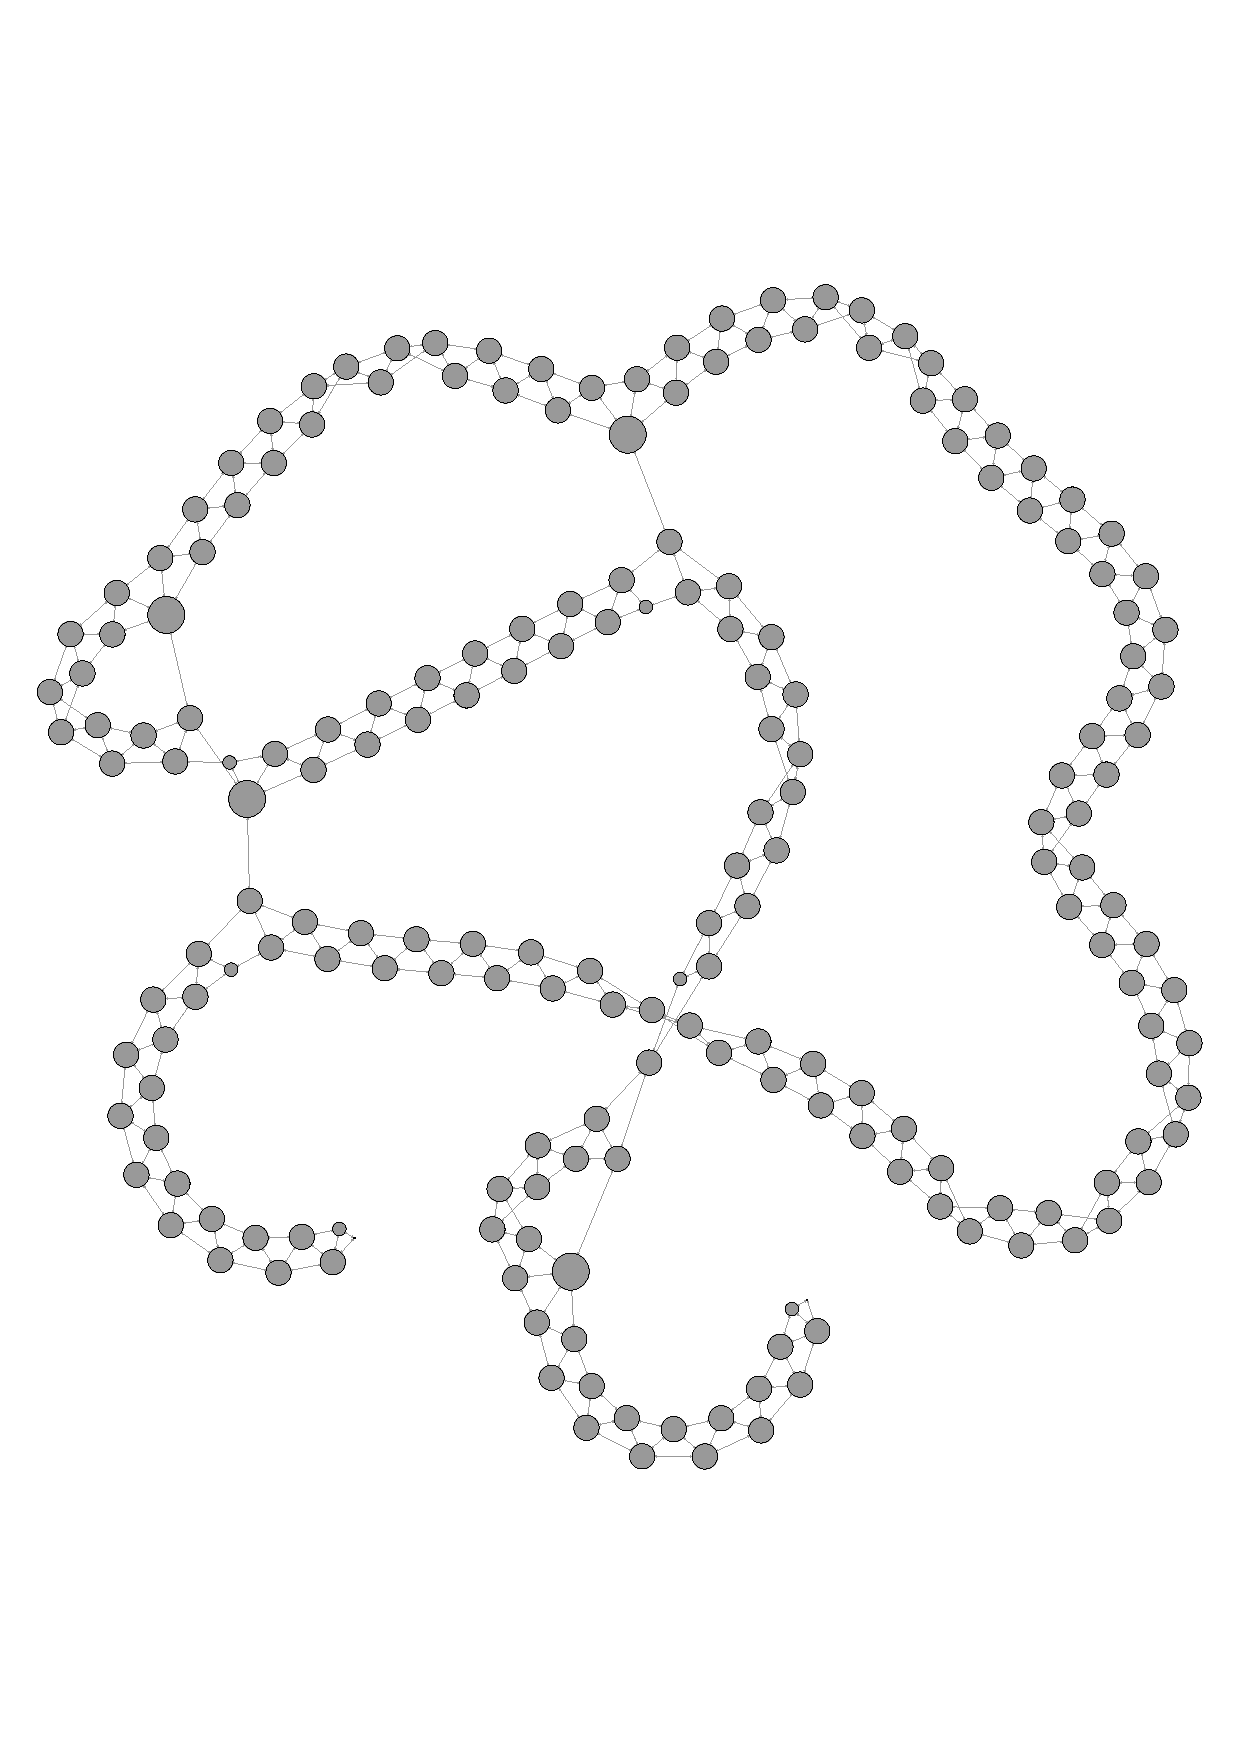
\includegraphics[width=2.5cm]{images//g00.pdf}\\
		$A\approx4$&
		\includegraphics[width=2.5cm]{images/g42.pdf}&
		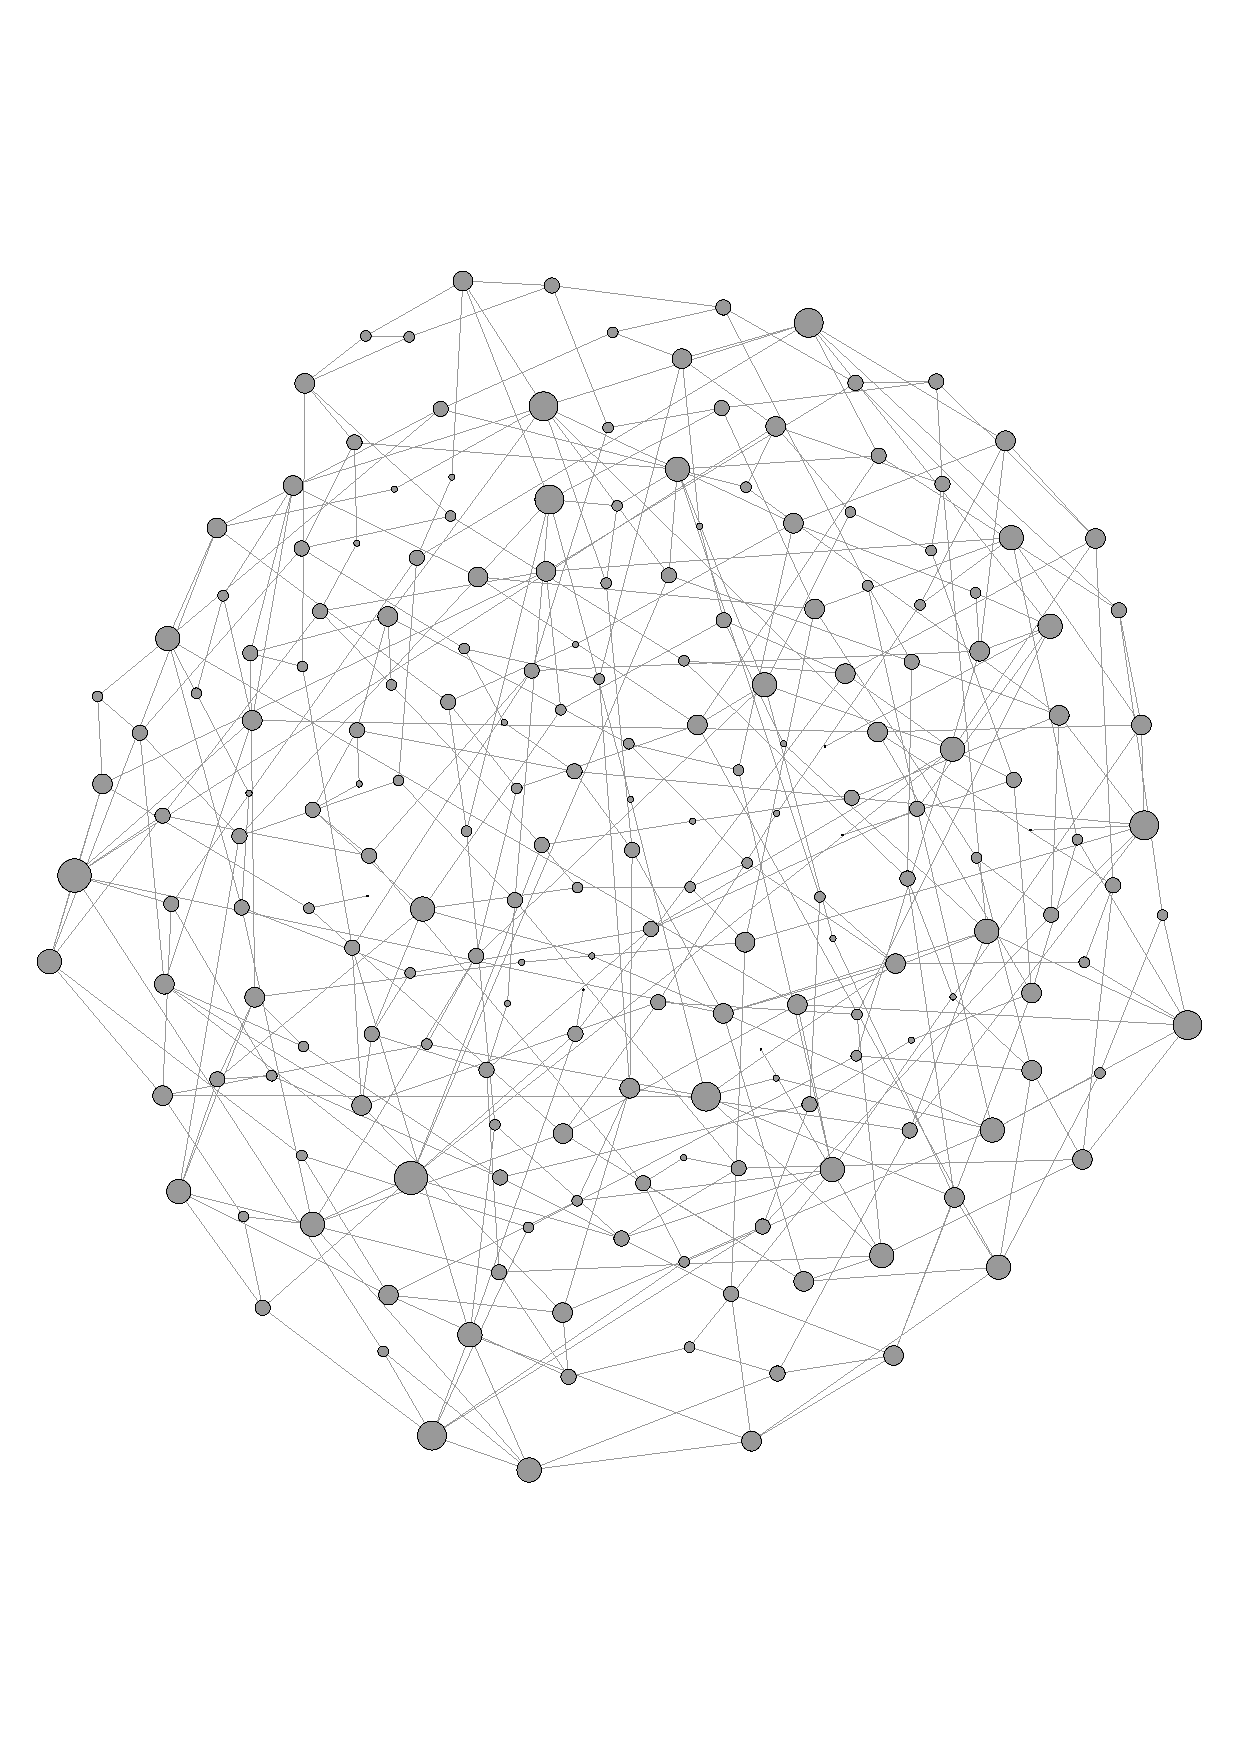
\includegraphics[width=2.5cm]{images/g40.pdf}\\
	\end{tabular}
    \end{table}
\end{frame}



\begin{frame}{Results: }
    \begin{figure}[h]
	\begin{center}
	    \includegraphics[height=.4\textheight]{images/densRes.pdf}\\
	    \includegraphics[height=.4\textheight]{images/distRes.pdf}
	\end{center}
	\label{fig:meancurve}
    \end{figure}

\end{frame}
    



\begin{frame}{Summary}
\begin{itemize}
	\item A local copy mechanism alone is enough to bring the global economy to an optimal equilibrium.
		\vfill
	\item The topology of the network where this copy mechanism occure influence the dynamics of the system
		\vfill
\end{itemize}

\end{frame}

%\section{Application}
%\begin{frame}{Case Study}
%	Roman Empire Economy: \\
%	Tight link between economy and culture, trace of it. \\
%	\begin{figure}
%		\includegraphics[width=.6\textwidth]{images/dressel-filiation.jpg}
%	\end{figure}
%	
%\end{frame}
%
%\begin{frame}{Case Study}
%	Simulation as a tool to implement and test Historical Hypothesis.
%	\begin{itemize}
%	\item Network Constraints
%	\item Temporal Constraints
%	\item Different Cultural Mechanisms
%	\end{itemize}
%\end{frame}
\begin{frame}{}
    \begin{center}
	\huge
	Thank for you attention!\\\vfill
	\includegraphics[width=2cm]{images/LOGO-ERC.jpg} \hfil	\includegraphics[width=3cm]{images/epnetLogo.png}\\
		\vspace{1cm}
		\scriptsize
			http://www.roman-ep.net/\\
			@epnetproject\\
			fb.com/EPNetProject\\
			@simoncarrignon
	\end{center}


\end{frame}

\end{document}


